\documentclass[a4paper, 12pt]{article}
\usepackage[T2A]{fontenc}
\usepackage[utf8]{inputenc}
\usepackage[english,russian]{babel}
\usepackage{amsmath, amsfonts, amssymb, amsthm, mathtools, misccorr, indentfirst, multirow}
\usepackage{wrapfig}
\usepackage{graphicx}
\usepackage{subfig}
\usepackage{enumitem}
\usepackage{adjustbox}
\usepackage{pgfplots}

\usepackage{geometry}
\geometry{top=20mm}
\geometry{bottom=20mm}
\geometry{left=20mm}
\geometry{right=20mm}
\newcommand{\angstrom}{\textup{\AA}}
\begin{document}
	\begin{titlepage}
		\begin{center}
		МИНИСТЕРСТВО ОБРАЗОВАНИЯ И НАУКИ РОССИЙСКОЙ ФЕДЕРАЦИИ\\
		\footnotesize{Московский физико-технический институт}\\
		\footnotesize{(государственный университет)}\\
		\vfill
		{\LARGE
		\textbf{Использование YAG:Nd$^{3+} $-лазера для гравировки материалов}\\
		}
		\vspace{1cm}
		Лабораторная работа по курсу\\
		фотоника
		\vfill
		\begin{flushright}
			Выполнили: студенты 654 и 653 групп.\\
			Нехаев А.С.\\
			Суманова Е.Д.\\
			Тихонов С.С.\\
			Хисматулина Е.А.\\
			Карпова Т.К.
		\end{flushright}
		\vfill
		г. Долгопрудный\\
		\the\year\:год
		\end{center}
	\end{titlepage}
	\newpage
	\pagenumbering{arabic}
	\tableofcontents
	\newpage
	\section{Цели и задачи исследования}
	\begin{enumerate}
		\item Изучить физические основы работы лазера в непрерывном режиме и режиме модуляции добротности;
		\item Исследовать зависимость мощности излучения от мощности накачки в режимах свободной генерации и модуляции добротности, т.е. найти КПД лазера в разных режимах работы;
		\item Исследовать зависимость ширины импульса от мощности накачки;
		\item Выгравировать изображение на пластиковой поверхности.	
	\end{enumerate}
	\newpage
	\section{Схема установки}
	\begin{figure}[h!]
	\begin{center}
		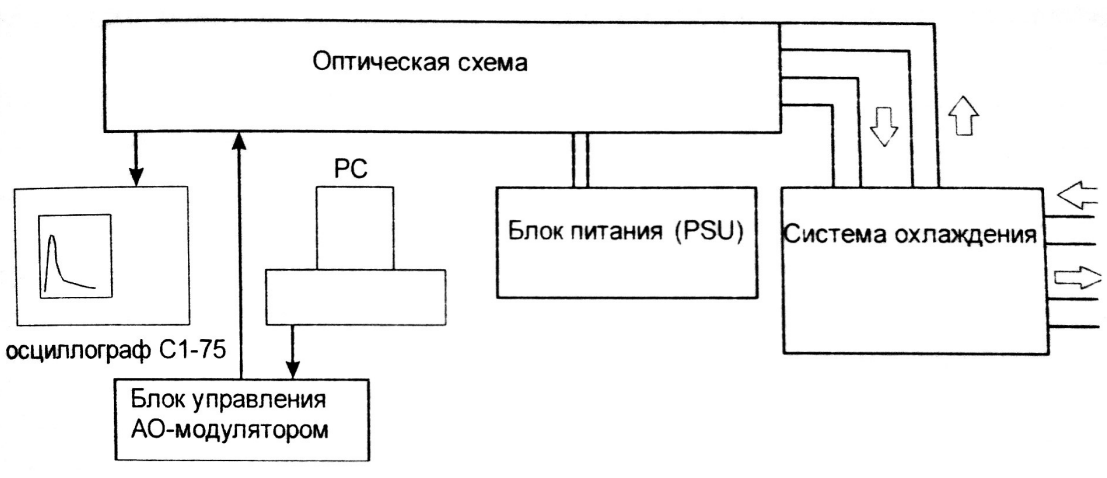
\includegraphics[scale = 0.4]{sch1}
		\caption{Принципиальная схема установки}
		\label{ris:shem1}
	\end{center}	
	\end{figure}
	\begin{figure}[h!]
	\begin{center}
		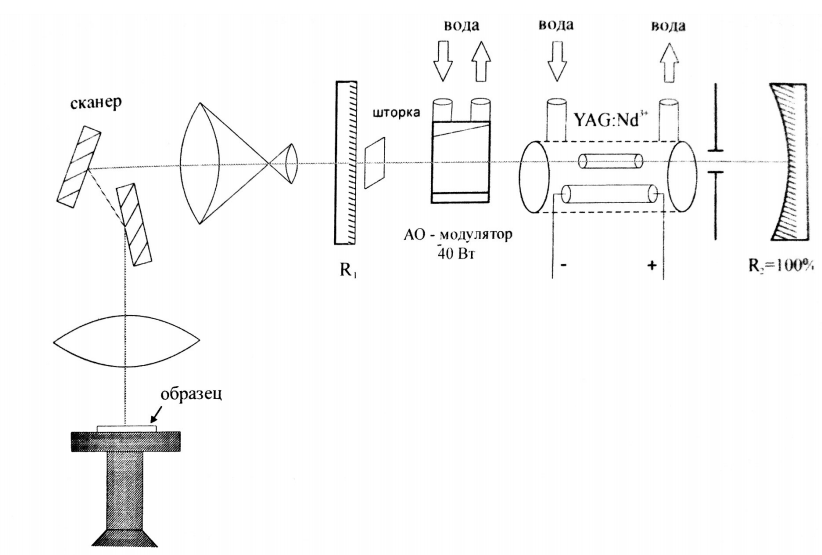
\includegraphics[scale = 0.44]{sch2}
		\caption{Схема оптической части}
		\label{ris:shem2}
	\end{center}	
	\end{figure}
	\section{Теоретичесое введение}
	
	В основе гравировки лазером лежит его тепловое воздействие на материал. При этом может происходить нагревание, плавление и испарение материала. Распределение тепла по материалу описывается уравнением теплопроводности, соответственно, к веществам с малым коэффициентом теплопроводности (например, металлам) необходимо применять короткоимпульсные лазеры, чтобы не взаимодействовать только с той областью материала, на которую попадает излучение. Отверстие наилучшей формы образуется в случае, если фокус лазера находится на поверхности материала. В этом случае определяющим процессом является испарение (рост отверстия вглубь), а ролью плавления (роста отверстия в ширину) можно пренебречь.\par
Описывать работу лазера принято \textit{скоростными уравнениями}:

\begin{equation}
\dfrac{dN}{dt} = R_p - B\phi N - \dfrac{N}{\tau},\quad
\dfrac{d\phi}{dt} = \left[BV_aN - \dfrac{1}{\tau_c}\right]\phi.
\label{eq_speed2}
\end{equation}
\par
Первое уравнение описывает изменение инверсии населённости, которое происходит из-за накачки, вынужденного и спонтанного излучений соответственно. Второе уравнение описывает изменение числа фотонов в резонаторе, обусловленное спонтанным излучением и временем жизни фотона в резонаторе.\par
В случае режима свободной генерации оба этих параметра принимают стационарные значения.
При модуляции добротности в лазере используется акустооптический модулятор, препятствующий генерации излучения путём увеличения потерь. Закрытый модулятор позволяет увеличивать рост инверсии заселённостей, а после открытия модулятора происходит генерация и резкое увеличесние числа фотонов в резонаторе. Таким образом, лазер может генерировать излучение в виде импульсов с большой пиковой мощностью, а из-за малой длительности импульса можно получить большую плотность мощности, что используется в обработке тугоплавких материалов.
\section{Результаты эксперимента}
\begin{table}[!htb]
	\centering
	\caption{Результаты измерений для режима свободной генерации.}
	\begin{tabular}{|c|c|c|c|}
	\hline
	Ток, А & Напряжение, В & Мощность накачки, мВт & Входная мощность, Вт\\
	\hline
 14.6 & 167. & 2. & 2438.2\\
 14.7 & 167. & 11. & 2454.9\\
 14.8 & 167. & 23. & 2471.6\\
 14.9 & 168. & 38. & 2503.2\\
 15. & 168. & 54. & 2520.\\
 15.1 & 168. & 72. & 2536.8\\
 15.2 & 169. & 95. & 2568.8\\
 15.3 & 169. & 116. & 2585.7\\
 15.4 & 169. & 131. & 2602.6\\
 15.5 & 170. & 152. & 2635.\\
 15.6 & 170. & 170. & 2652.\\
 15.7 & 170. & 194. & 2669.\\
 15.8 & 171. & 218. & 2701.8\\
 15.9 & 171. & 254. & 2718.9\\
 16. & 171. & 284. & 2736.\\
 16.1 & 172. & 320. & 2769.2\\
 16.2 & 172. & 354. & 2786.4\\
 16.3 & 172. & 386. & 2803.6\\
 16.4 & 173. & 425. & 2837.2\\
 16.5 & 173. & 464. & 2854.5\\
 16.6 & 173. & 490. & 2871.8\\
 16.7 & 174. & 538. & 2905.8\\
 16.8 & 174. & 599. & 2923.2\\
 16.9 & 175. & 642. & 2957.5\\
 17. & 175. & 690. & 2975.\\
 17.1 & 176. & 736. & 3009.6\\
 17.2 & 176. & 790. & 3027.2\\
 17.3 & 176. & 835. & 3044.8\\
 17.4 & 177. & 884. & 3079.8\\
 \hline
	\end{tabular}
\end{table}
\begin{table}[!htb]
	\centering
	\caption{Результаты измерений для режима модуляции добротности.}
	\begin{tabular}{|c|c|c|c|}
	\hline
	Ток, А & Напряжение, В & Мощность накачки, мВт & Входная мощность, Вт\\
	\hline
 14.4 & 167. & 2. & 2404.8 \\
 14.5 & 167. & 14. & 2421.5 \\
 14.6 & 168. & 35. & 2452.8 \\
 14.7 & 168. & 51. & 2469.6 \\
 14.8 & 168. & 69. & 2486.4 \\
 14.9 & 169. & 85. & 2518.1 \\
 15. & 169. & 102. & 2535. \\
 15.1 & 169. & 121. & 2551.9 \\
 15.2 & 170. & 140. & 2584. \\
 15.3 & 170. & 161. & 2601. \\
 15.4 & 170. & 182. & 2618. \\
 15.5 & 171. & 203. & 2650.5 \\
 15.6 & 171. & 232. & 2667.6 \\
 15.7 & 171. & 257. & 2684.7 \\
 15.8 & 172. & 284. & 2717.6 \\
 15.9 & 172. & 297. & 2734.8 \\
 16. & 172. & 325. & 2752. \\
 16.1 & 172. & 357. & 2769.2 \\
 16.2 & 173. & 397. & 2802.6 \\
 16.3 & 173. & 432. & 2819.9 \\
 16.4 & 174. & 470. & 2853.6 \\
 16.5 & 174. & 511. & 2871. \\
 16.6 & 174. & 531. & 2888.4 \\
 16.7 & 174. & 562. & 2905.8 \\
 16.8 & 175. & 602. & 2940. \\
 16.9 & 175. & 641. & 2957.5 \\
 17. & 175. & 686. & 2975. \\
 17.1 & 176. & 727. & 3009.6 \\
 17.2 & 176. & 772. & 3027.2 \\
 17.3 & 176. & 810. & 3044.8 \\
 17.4 & 177. & 854. & 3079.8 \\
 \hline
	\end{tabular}
\end{table}
\begin{figure}[!h]
	\minipage{0.48\textwidth}
	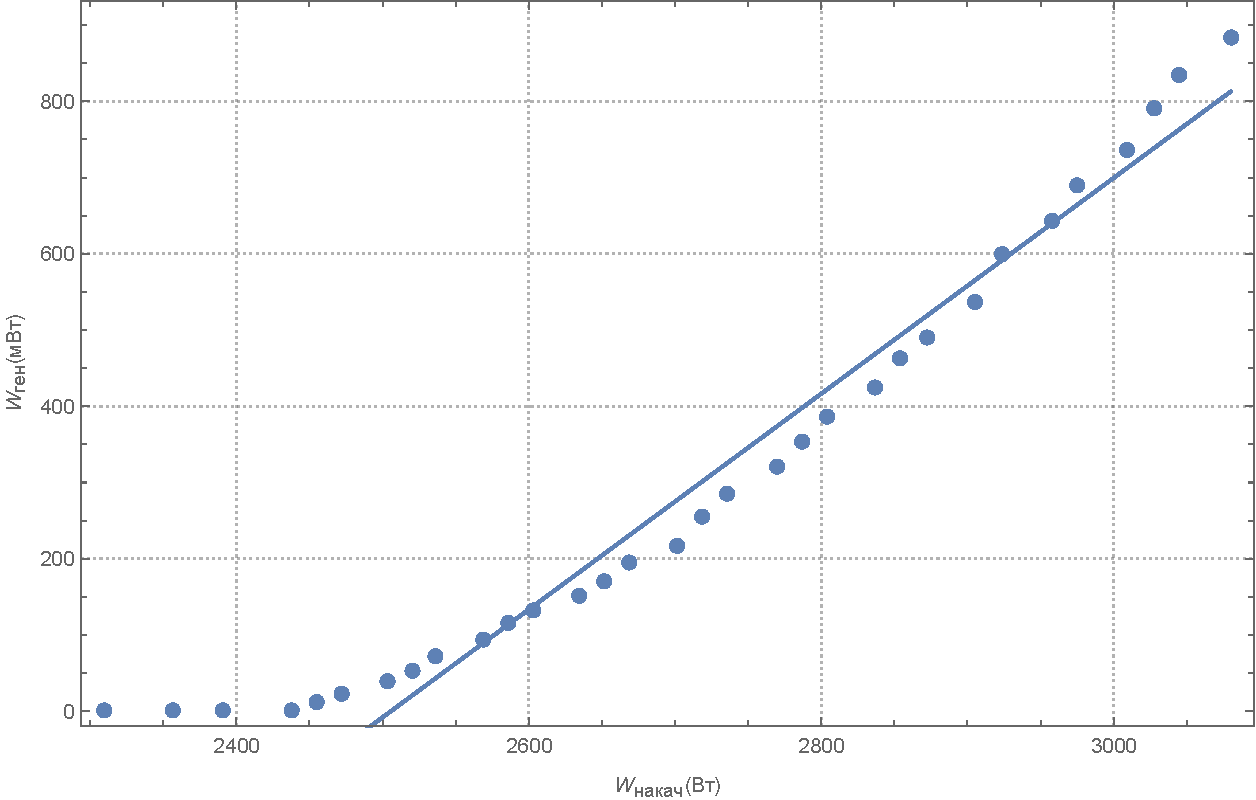
\includegraphics[width=\textwidth]{1.pdf}
	\caption{Зависимость мощности излучения от мощности накачки в режиме свободной генерации}
	\endminipage
	\hfill
	\minipage{0.48\textwidth}
	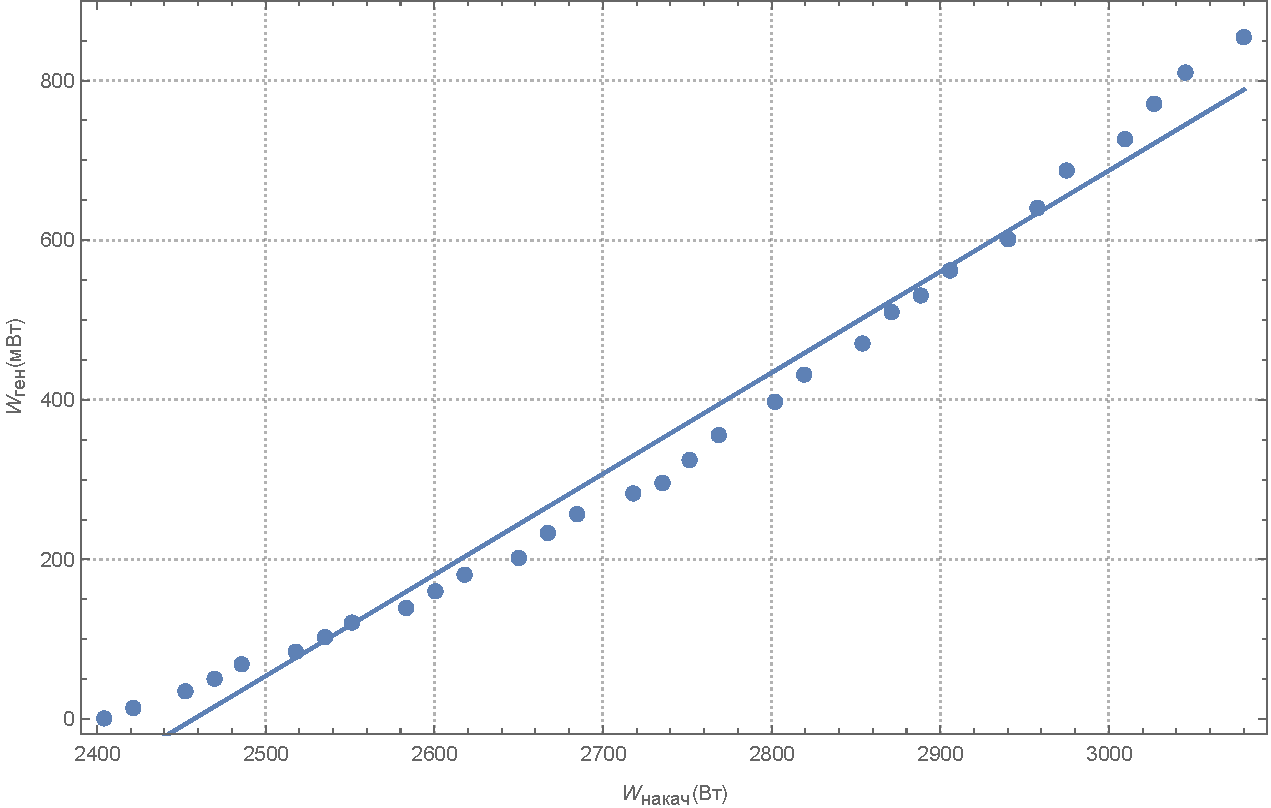
\includegraphics[width=\textwidth]{2.pdf}
	\caption{Зависимость мощности излучения от мощности накачки в режиме модуляции добротности}
	\endminipage
\end{figure}
По графикам определим КПД лазера в разных режимах работы, как угловой коэффициент наклона аппроксимирующей прямой:
$ \eta_{CW} \approx (0,14 \pm 0,02)\% $ и 
$ \eta_{QW} \approx (0,13 \pm 0,02)\% $. Также определим пороговую мощность 
$ W_{CW} \approx (2505 \pm 125) $ Вт и 
$ W_{CW} \approx (2457 \pm 95) $ Вт соответственно.
\begin{table}[!htb]
	\centering
	\caption{Результаты измерения зависимости длительности импульса от мощности накачки лазера в режиме модуляции добротности.}
	\begin{tabular}{|c|c|c|c|}
		\hline
		$I$, А & $U$, В & $t$, мкс & $W$, Вт\\
		\hline
		17.4 & 177. & 0.38 & 3079.8 \\
 17.2 & 176. & 0.33 & 3027.2 \\
 17. & 176. & 0.34 & 2992. \\
 16.8 & 175. & 0.34 & 2940. \\
 16.6 & 175. & 0.38 & 2905. \\
 16.4 & 174. & 0.42 & 2853.6 \\
 16.2 & 173. & 0.34 & 2802.6 \\
 16. & 173. & 0.37 & 2768. \\
 15.8 & 172. & 0.42 & 2717.6 \\
 15.6 & 171. & 0.45 & 2667.6 \\
 15.4 & 170. & 0.54 & 2618. \\
 15.2 & 170. & 0.52 & 2584. \\
 15. & 169. & 0.56 & 2535. \\
 14.8 & 169. & 0.7 & 2501.2 \\
 14.6 & 168. & 0.84 & 2452.8 \\
 \hline
	\end{tabular}
\end{table}
\begin{figure}[!htb]
	\centering
	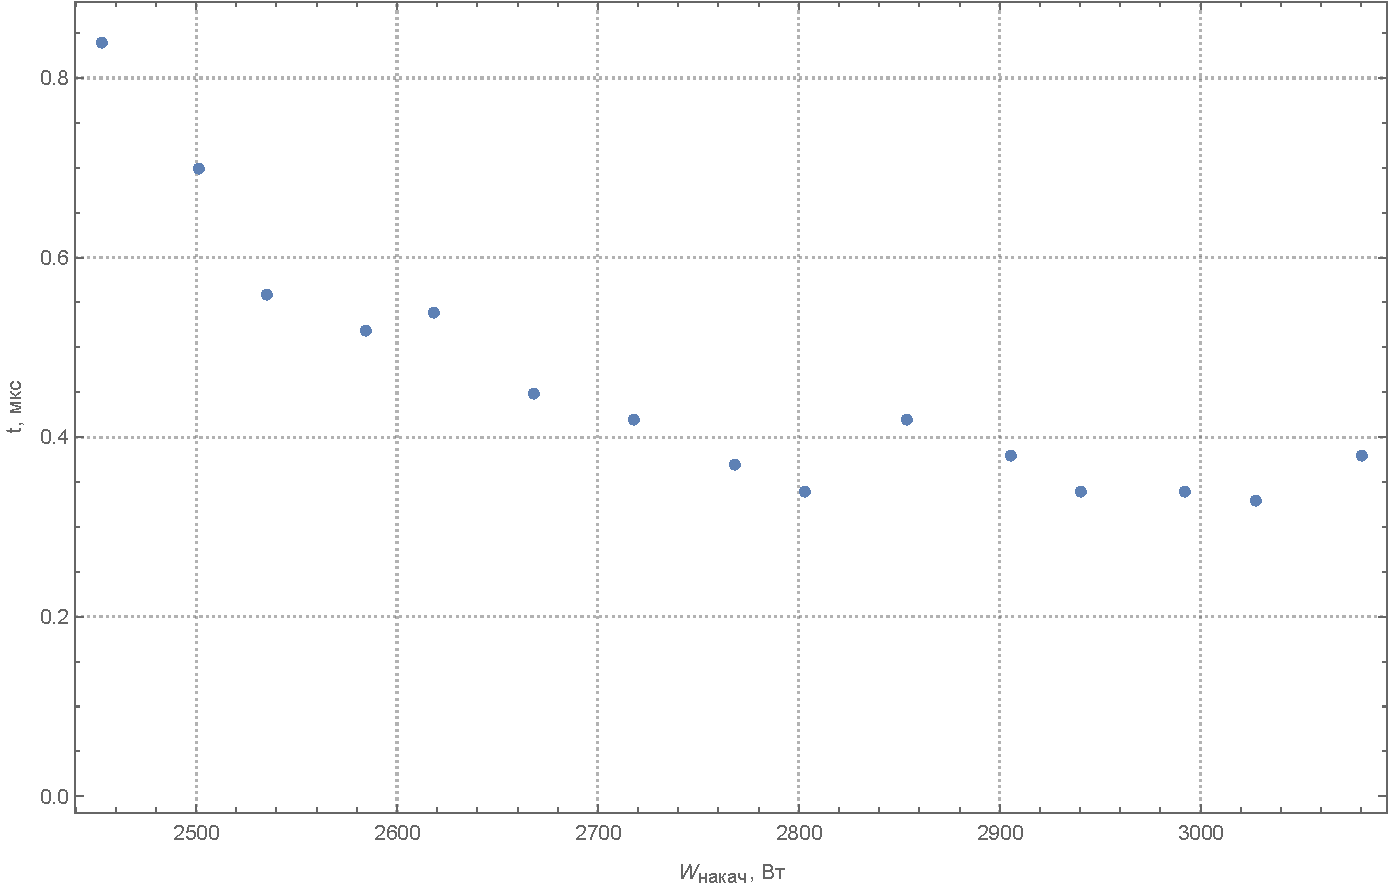
\includegraphics[width=\textwidth]{3.pdf}
	\caption{График зависимости длительности импульса от мощности накачки}
\end{figure}
\section{Гравировка изображения}
Для демонстрации технических возможностей лазера была произведена гравировка изображения.
\begin{figure}[!htb]
	\centering
	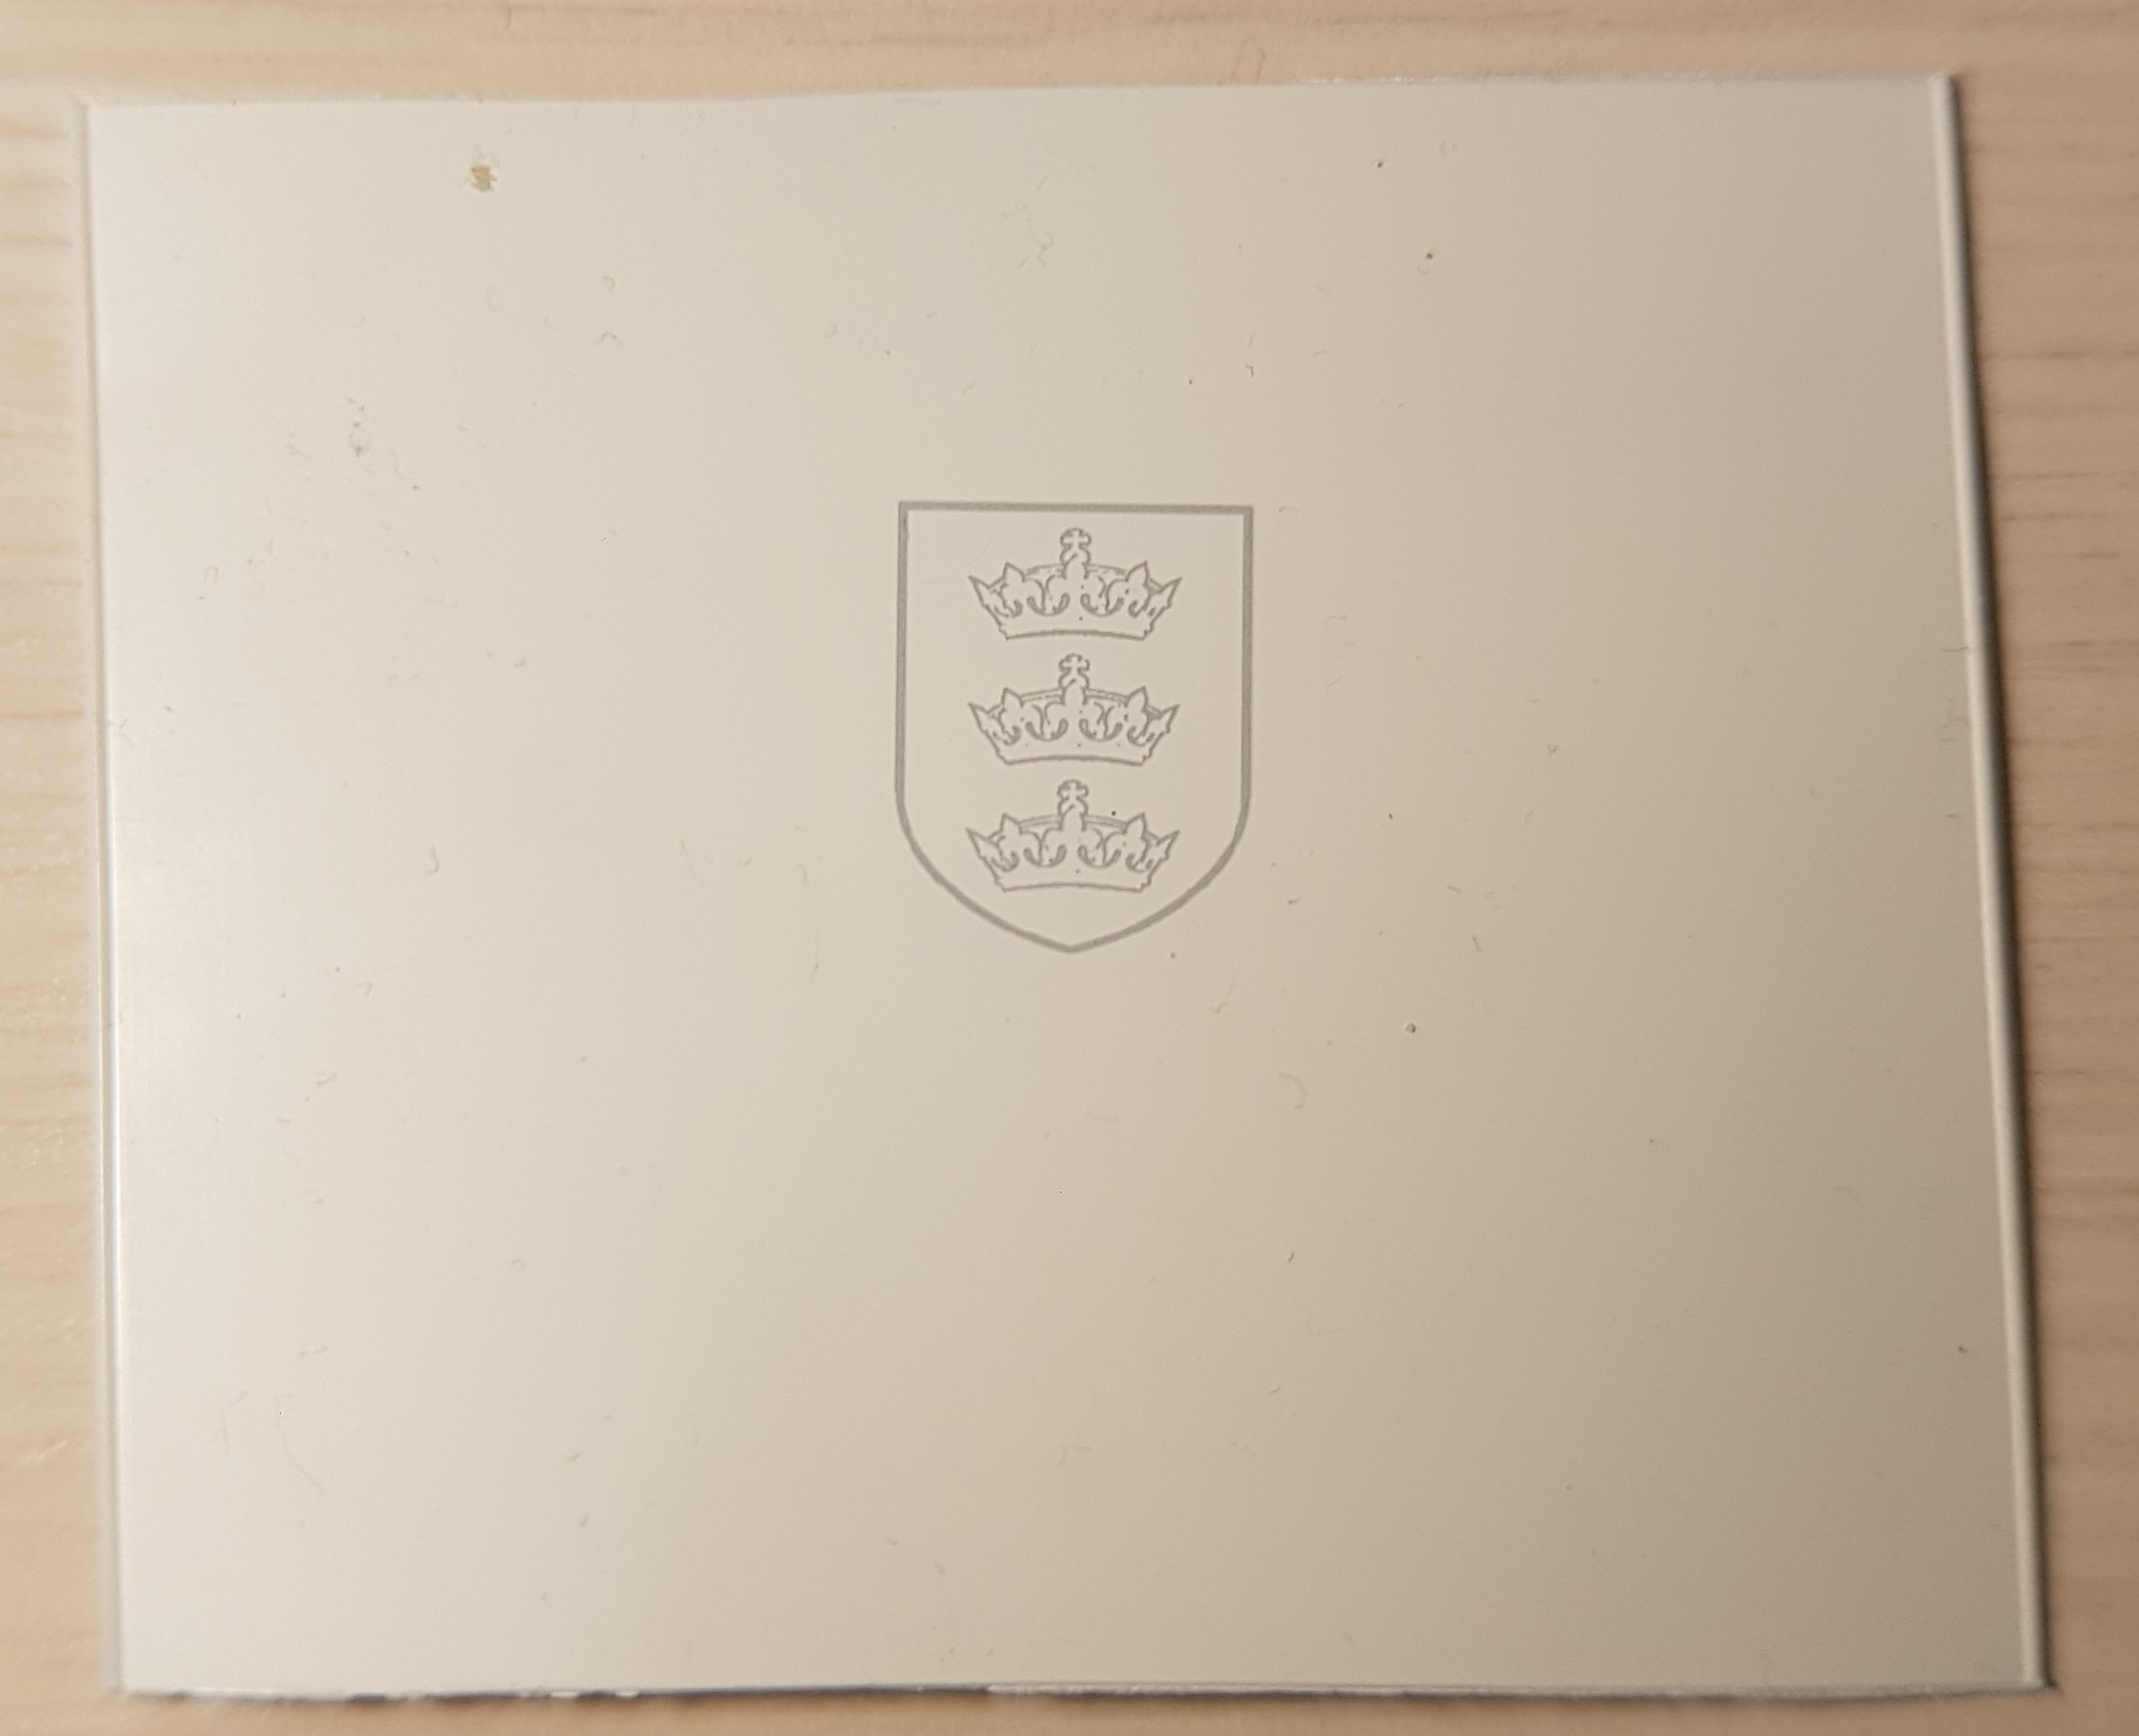
\includegraphics[scale=0.12]{card.jpg}
	\caption{Выгравированное изображение}
\end{figure}
\section{Вывод}
Были изучены физические основы работы различных режимов лазера и определены КПД и пороговая мощность:
\begin{table}[h!]
		\centering
		\begin{tabular}{|c||c|c|}
			\hline
			Режим & Свободной генерации   & Модуляции добротности \\ 					\hline
			$\eta$,~\%   & 0,14 & 0,13 \\ \hline
			$P_{\text{пор}}$, Вт    & 2505 & 2457 \\
			\hline
		\end{tabular}
	\end{table}\par
	В режиме модуляции добротности КПД лазера меньше, чем в непрерывном режиме. Это связано с тем, что в режиме модуляции добротности инверсная населённость в среднем больше (потому что в данном случае отсутствует вынужденное излучение при закрытом модуляторе), чем в непрерывном режиме, а значит, больше потери на спонтанное излучение.\par
	При достижении пороговой мощности усиление в активной среде становится равным потерям в резонаторе, поэтому пороговая мощность не должна зависеть от режима работы. Это и было получено в работе, так как мощности оказались равны в пределах погрешности.
\end{document}